\documentclass[10pt,table,dvipsnames]{beamer}

\usepackage{tikz}

\usepackage[absolute,overlay]{textpos}
\author{C.~Grefe, \underline{S.~Poss}, A.~Sailer}
\title{ILCDIRAC}
\subtitle{A grid solution for the LC community}
\date[Oct. 1st 2013, CLIC dp meeting]{October 1st, 2013\\CLIC detectors \& physics meeting}
\institute{CERN}
\newcommand{\interstitial}[1]{\begin{frame}\begin{block}{}\centering\Huge{#1}\end{block} \end{frame}}
\newcommand{\backupslides}{\interstitial{Backup Slides}}

\mode<all>
\TPGrid{50}{50}

\pgfdeclareimage[width=0.1\paperwidth]{cliclogo}{CLIClogo}
\newcommand{\ClicLogo}{%
\begin{textblock}{14}(45., 0.05)
 \href{http://lcd.web.cern.ch}{\pgfuseimage{cliclogo}}
\end{textblock}
}

\setbeamertemplate{footline}
{%
  \leavevmode%
  \hbox{%
  \begin{beamercolorbox}[wd=.222222\paperwidth,ht=2.25ex,dp=1ex,left]{title in 
head/foot}%
    \usebeamerfont{date in head/foot}\insertshortdate{}\hspace*{2em}
  \end{beamercolorbox}%
  \begin{beamercolorbox}[wd=.555555\paperwidth,ht=2.25ex,dp=1ex,center]{author 
in head/foot}%
    \usebeamerfont{author in head/foot}\insertshortauthor{}:
    \usebeamerfont{title in head/foot}\insertshorttitle
  \end{beamercolorbox}%
  \begin{beamercolorbox}[wd=.222222\paperwidth,ht=2.25ex,dp=1ex,right]{date in 
head/foot}%
    \insertframenumber{}/\inserttotalframenumber\hspace*{2ex}
  \end{beamercolorbox}}%
  %\vskip0pt%
  \ClicLogo
}
\beamertemplatenavigationsymbolsempty 
\setbeamertemplate{blocks}[rectangle]
\setbeamersize{text margin left=1em,text margin right=1em}

%\setbeamertemplate{headline}[default]

\begin{document}
\renewcommand{\inserttotalframenumber}{\ref{lastframe}}
\begin{frame}
\titlepage
\end{frame}

\begin{frame}
\frametitle{Outline}
\tableofcontents
\end{frame}

\section{Current status}
\begin{frame}
\frametitle{Current status}
\alert{ILCDIRAC now stable}, no more major developments, only bug fixes.

~\\

ILD concept now moves towards using ILCDIRAC:
\begin{itemize}
\item Used it for user jobs
\item Several questions came
\item ILCDIRAC required a few fixes to adapt to that use case: Production job class, support for application specific inputs (ILDConfig package)
\item File Catalog meta data adjustements required for ILD
\item The web interface to the File Catalog has issues (DIRAC, not ILCDIRAC), but working on those now. Next major version of the portal will have a different interface.
\end{itemize}
Eduard Avetisyan\footnote{\url{http://ilcagenda.linearcollider.org/conferenceOtherViews.py?view=standard&confId=6113}}:
\begin{quote}
"ILCDIRAC is an appropriate system for future ILD productions"
\end{quote}
More users are coming every week, now $\approx 100$ registered, 20 active
\end{frame}

\begin{frame}
\frametitle{Current status: User jobs}
\centering
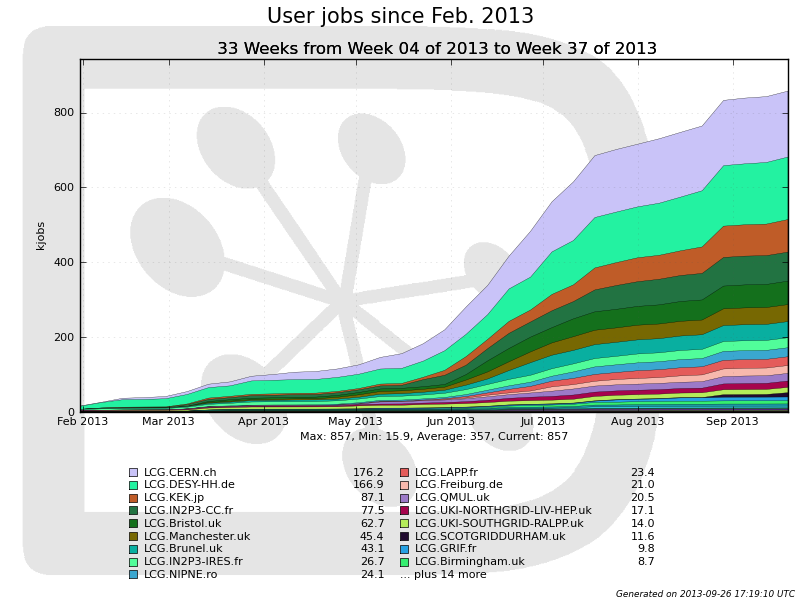
\includegraphics[width=0.9\textwidth]{userjobs}
\end{frame}
\begin{frame}
\frametitle{Current status: User jobs}
\centering
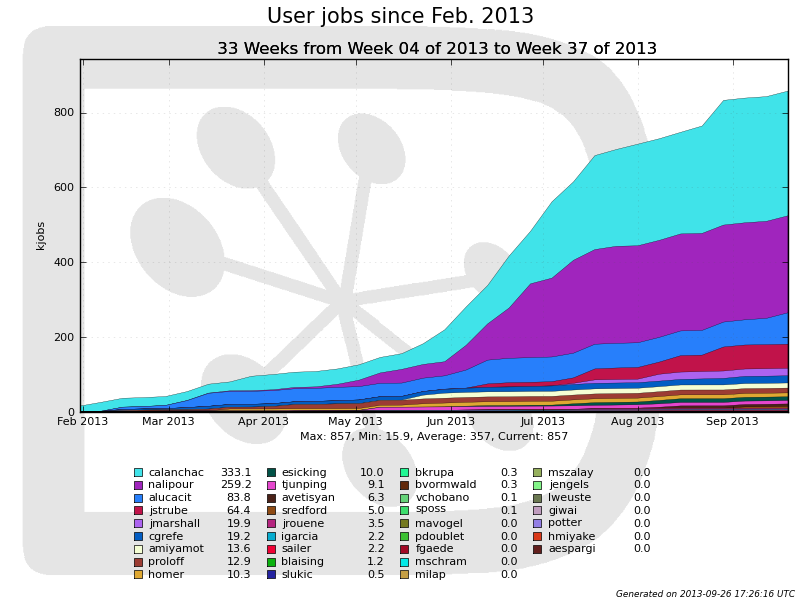
\includegraphics[width=0.9\textwidth]{userjobsperuser}
\end{frame}
\begin{frame}
\frametitle{Current status: User jobs}
\centering
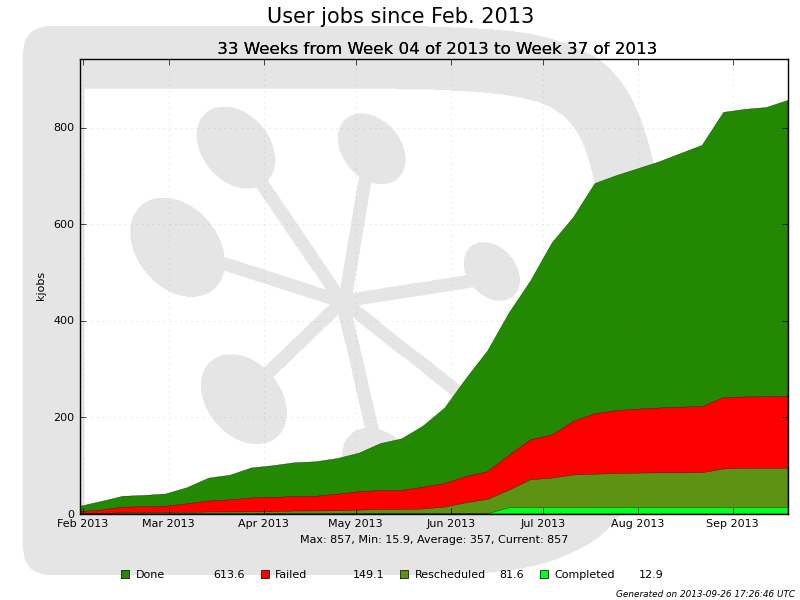
\includegraphics[width=0.9\textwidth]{userjobsperstatus}
\end{frame}

\begin{frame} 
\frametitle{Current status: Production jobs}
\centering
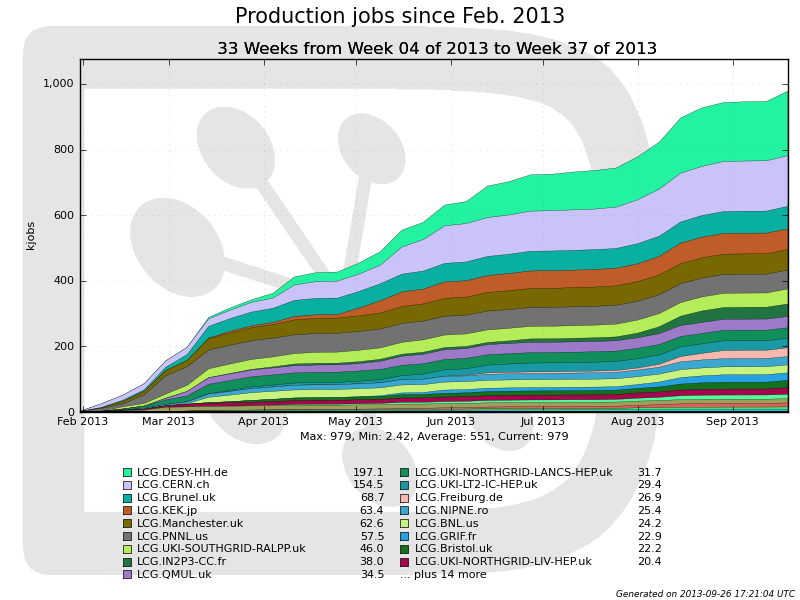
\includegraphics[width=0.9\textwidth]{prodjobs}
\end{frame}

\begin{frame} 
\frametitle{Current status: All jobs}
\centering
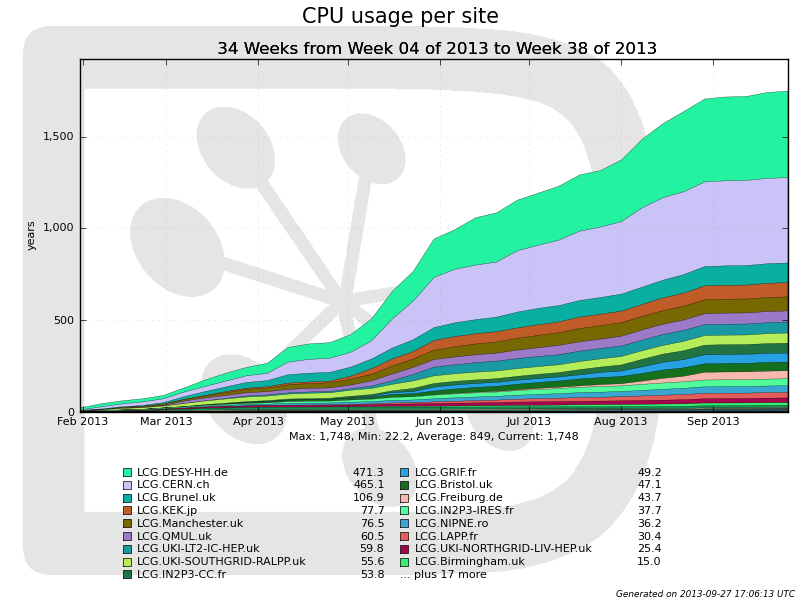
\includegraphics[width=0.9\textwidth]{CPUPerSite}
\end{frame} 

\section{Data management}
\begin{frame}
\frametitle{Data management}
DIRAC File catalog (DFC) knows about:
\begin{itemize}
\item most files produced for the ILC DBD
\item all files for the SID DBD
\item all files for CLIC
\end{itemize}
Lcg File Catalog and DFC are written in parallel, and
thanks to the failover mechanism: \alert{NO DATA LOSS}

~\\

Storage elements:
\begin{itemize}
\item Failover mechanism also protects physical files: automatic replications between sites
\item Top 5 storage element usage {\scriptsize (FC:/$>$size -l)}:\\
\begin{center}
\begin{tabular}{|ccccc|}
\hline
Storage & Usage & CLIC & ILC & Files \\
\hline
CERN-SRM & 868 TB & 861 TB & 7 TB & 4\,053\,817\\
\hline
DESY & 96 TB & 0 & 96 TB& 306\,585\\
\hline
KEK & 95 TB & 76 GB & 94 TB & 244\,148\\
\hline
RAL-SRM & 93 TB & 4TB & 89 TB & 1\,026\,781\\
\hline
PNNL-SRM & 25 TB & 0 & 25 TB & 733\,423\\
\hline
\end{tabular}
\end{center}
Most data produced for the CLIC CDR.
\end{itemize}

\end{frame}

\section{Bug tracking}
\begin{frame}
\frametitle{Bug tracking}
Use of JIRA: \url{http://its.cern.ch/jira/browse/ILCDIRAC}
\begin{center}
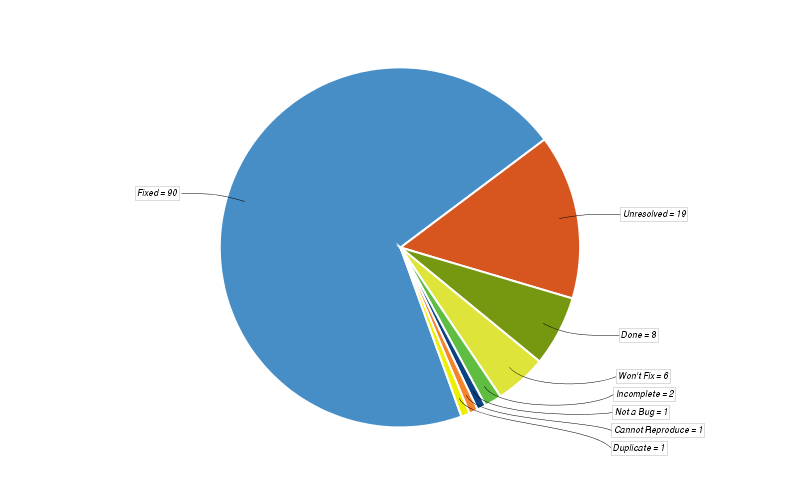
\includegraphics[width=0.8\textwidth]{charts_1}
\end{center}
\end{frame}
\begin{frame}
\frametitle{Bug tracking}
From Web portal:
\centering
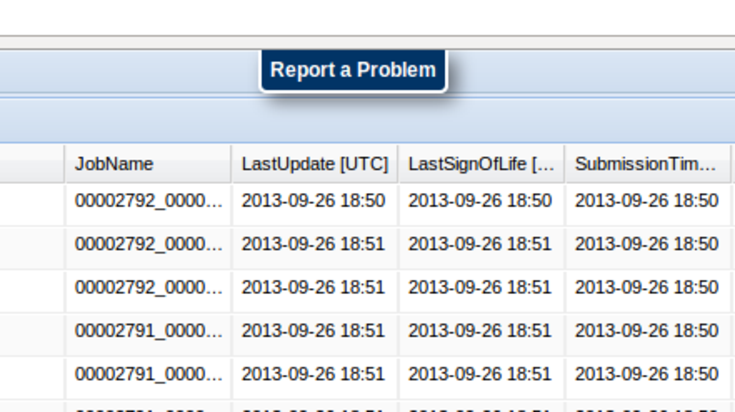
\includegraphics[width=0.9\textwidth]{ReportProb} 
\end{frame}

\section{Contact info}
\begin{frame}
\frametitle{Mailing lists}
Register: \url{ilcdirac-register@cern.ch}

~\\

Questions: \url{ilcdirac-support@cern.ch}

~\\

Forum: {\small \url{http://forum.linearcollider.org/index.php?t=index&cat=22&rid=0}}

~\\

Information: {\small\url{https://twiki.cern.ch/twiki/bin/view/CLIC/DiracUsage}}
\vfill
\begin{center}
\alert{\Large Any new user is welcome!}
\end{center}

\end{frame} 

\section{Final word}
\begin{frame}
\frametitle{Thanks}

Our thanks go to 
\begin{itemize}
\item the Site administrators for fixing the issues quickly
\item the DIRAC developers for fast replies and discussions
\item the users for positive feedback
\end{itemize}

\label{lastframe}
\end{frame} 

\end{document}


% Local Variables:
% TeX-PDF-mode: t
% End:
